\documentclass[11pt,a4paper]{article}
\usepackage[T1]{fontenc}
\usepackage{lmodern}
\usepackage{amsmath,amssymb,amsthm,mathtools}
\usepackage{booktabs,tabularx,array,graphicx}
\usepackage{float}
\usepackage{tikz}
\usetikzlibrary{arrows.meta,positioning,calc,fit}
\usepackage{geometry}
\usepackage{microtype}
\usepackage{setspace}
\usepackage{natbib}
\usepackage{hyperref}
\geometry{margin=1in}
\setstretch{1.12}
\hypersetup{colorlinks=true,linkcolor=blue,citecolor=blue,urlcolor=blue}
\newtheorem{theorem}{Theorem}
\newtheorem{proposition}[theorem]{Proposition}
\newtheorem{lemma}[theorem]{Lemma}
\newtheorem{corollary}[theorem]{Corollary}
\theoremstyle{remark}\newtheorem{remark}[theorem]{Remark}
\newcommand{\SW}{\mathrm{SW}}\newcommand{\SU}{\mathrm{SU}}\newcommand{\IS}{\mathrm{IS}}
\newcommand{\N}{\mathrm{N}}\newcommand{\F}{\mathrm{F}}
\newcommand{\loss}{\mathcal L}\newcommand{\vect}[1]{\boldsymbol{#1}}
\title{Endogenous Product Design and Participation in\\ International Compatibility Agreements}
\author{Review working draft---author details withheld}
\date{22 October 2026\quad |\quad Stage 25, version 0.4\quad |\quad \textbf{Not for submission}}
\begin{document}
\maketitle
\begin{abstract}
Can privately optimal product redesign overturn governments' incentives to join an international compatibility agreement? We develop a three-country model in which governments choose bilateral or multilateral compatibility arrangements, firms subsequently choose residual product characteristics in Nash equilibrium, and production takes place in Cournot markets with network effects. Holding the governmental accession protocol fixed, we compare endogenous design with a benchmark that freezes firms' characteristics at their no-agreement levels. A national-welfare decomposition isolates the direct gain from an agreement and the induced loss arising from private redesign. Under explicit sufficient conditions the latter reverses both an initial member's participation incentive and an outsider's accession incentive. A certified nonempty open set of primitive parameters supports a stronger equilibrium contrast: positive-depth multilateral coordination is chosen with fixed design but the sequential-accession game remains fragmented with endogenous design. Direct multilateral agreement can nevertheless improve every country's welfare. The fragmentation result is therefore conditional on an inherited-depth accession procedure, not an impossibility of cooperation under unrestricted bargaining. Adjustment costs and network intensity delineate additional, explicitly limited boundaries. We distinguish this design-incidence mechanism from previously established results on product-standard coalitions and regulatory cooperation.
\end{abstract}
\noindent\textbf{Keywords:} compatibility standards; endogenous product differentiation; national welfare; coalition accession; network externalities; Cournot competition; institutional commitment.\\
\textbf{JEL:} F13, F15, L13, L15, D62, C72.

\section{Introduction}
A common compatibility standard can increase the value of consumption across jurisdictions. Yet the policy that appears desirable with a fixed configuration of products need not remain politically acceptable after firms respond. Product developers can change the attributes left outside the standard, and those changes affect a government's domestic consumers and the profits of its firms in every destination market. A national government consequently evaluates a different payoff from the one implicit in an engineering-only comparison of compatible products.

We examine a question at the boundary of industrial organization and public economic theory: \emph{Can the noncooperative redesign of products, by itself, reverse national consent to a compatibility agreement when the government's menu of agreements has not changed?} A second question asks which part of the resulting noncooperation reflects private incentives, and which reflects the institutional route through which countries attempt to cooperate.

The distinction is subtle. Existing research has already shown that regional standard-setting can prevent globally attractive harmonization \citep{Takarada2020,Kawabata2021}; other work combines national product regulation with firms' endogenous attribute choices \citep{Grossman2021}. Endogenous compatibility choice and private veto effects are also familiar in network industries \citep{Buccella2023,Cheng2025}. Our contribution is \emph{not} the generic existence of incomplete standards coalitions, nor the idea that companies adapt products in response to regulation. We isolate an additional, model-specific \emph{national-incidence channel}: firms' residual-design Nash responses subtract from the direct national benefit of compatibility, and the subtraction can change the sign of government participation inequalities under precisely the same government accession rules.

To identify this channel, we hold constant demand, country welfare objectives, the possible compatibility link patterns, and the sequence of governmental offers. Only firms' subsequent design behavior differs across our principal comparison. We derive a transparent local decomposition,
\begin{equation}\label{eq:introheadline}
\left.\frac{\partial m_{\F}(g)}{\partial g}\right|_{g=0}=D>0,\qquad
\left.\frac{\partial m_{\N}(g)}{\partial g}\right|_{g=0}=D-\loss<0,
\end{equation}
where $m$ is a prospective bilateral member's national welfare, $D$ is the direct effect at fixed design, and $\loss$ is the incidence of firms' equilibrium redesign on domestic consumer surplus and home-firm worldwide profits. The private first-order condition does not set these national effects to zero. Exchangeability across three countries then transmits the same sign reversal to the outsider's incentive to join an existing bilateral arrangement.

A second result moves beyond a derivative at one point. Using independently checked equilibrium equations and existing rigorous interval certificates, we identify a nonempty \emph{open neighborhood} of primitive parameters in which all positive-depth proposals fail under the specified inherited-depth, bilateral-first procedure when product design is endogenous; with the same primitives and governmental procedure, freezing residual design yields an accepted, government-preferred multilateral agreement. A positive-depth direct grand agreement would nevertheless raise welfare in all three countries under endogenous design. Hence the failure is neither an engineering impossibility nor a general claim of coalition-proof fragmentation.

The institutional restriction is deliberate. The initial bilateral proposal specifies a compatibility depth that a later entrant may accept or reject but cannot revise in the same accession round. This separates accession to an existing specification from negotiation of a newly specified multilateral interface. Larger standard-setting committees can face distributive bargaining frictions \citep{Simcoe2012}; nevertheless, the model \emph{does not} prove that this procedure is endogenously optimal, that technical specifications cannot be amended in practice, or that direct multilateral negotiation is unavailable in every standards organization. The direct-proposal counterfactual is used expressly to reveal this limitation.

The paper uses a timing diagram, a causal sign-decomposition diagram, compact tables, and a carefully delimited numerical phase map to distinguish the economic mechanism from the domain of its proof. Our approach is a specialized public-economic-theory contribution: the causal mechanism concerns a national participation constraint, not the invention of a new oligopoly equilibrium concept. The strongest comparison is with government standards coalitions \citep{Takarada2020,Kawabata2021} and regulatory agreements involving privately chosen product characteristics \citep{Grossman2021}. Section~\ref{sec:model} defines the primitives; Sections~\ref{sec:equilibrium}--\ref{sec:global} derive the national-incidence channel and equilibrium contrast; Section~\ref{sec:institution} compares negotiation routes; Section~\ref{sec:boundaries} identifies the limits of cost and network-intensity results. Longer algebra and the verification map are collected in the Appendix.

\section{Economic environment and the accession protocol}\label{sec:model}
\subsection{Three countries, compatibility, and residual design}
There are three symmetric countries $A,B,C$, each with one firm. All three firms sell in each of three identical segmented national markets. Each firm chooses a residual product characteristic $x_i\in[0,1]$; a larger $x_i$ is a higher level of the model's residual attribute, and $1-x_i$ is the reverse scale of the \emph{same} attribute, not another decision variable. The compatibility arrangement is a separate government choice.

Let $g\in[0,1]$ denote the proposed depth of common compatibility and write $H$ for the country-link matrix: $H_{ii}=1$ and $H_{ij}=0$ under fragmentation $\SW$, $H_{AB}=H_{BA}=g$ with other off-diagonal entries zero under bilateral compatibility $\SU$, and $H_{ij}=g$ for every $i\ne j$ under integrated compatibility $\IS$. Define $X_{ii}=1$ and $X_{ij}=(x_i+x_j)/2$ for $i\ne j$. The cross-product matrix and fulfilled-expectations Cournot matrix are
\begin{equation}\label{eq:matrices}
B=\rho H+(1-\rho)X,\qquad M=I+B-\eta H,
\end{equation}
where $\rho$ is the weight placed on the government-specified compatibility component and $\eta$ is the strength of fulfilled network effects. In particular, $g$, $x_i$, and $\rho$ play different roles; they must not be interpreted as interchangeable measures of product differentiation.

For one destination market, an integrable quadratic consumer payoff yielding the inverse demands can be written, for fixed network expectations $\bar{q}$, as
\begin{equation}\label{eq:consumer}
U(q;\bar q)=(c+d)\vect{1}^{\top}q-\tfrac12q^{\top}Bq+\eta q^{\top}H\bar q,\qquad
p=(c+d)\vect{1}-Bq+\eta H\bar q.
\end{equation}
The matrix $B$ is symmetric. We maintain the regular range in which the underlying consumer problem and subsequent interior outputs are well-defined. Consumers and firms take network expectations as fixed during a unilateral quantity deviation; expectations are fulfilled at equilibrium. Every firm's constant marginal production cost is $c$ and $d>0$ is the net-demand intercept.

In the baseline, firm $i$ bears a one-time design cost
\begin{equation}\label{eq:cost}
K_i(x_i)=\tfrac{\kappa}{2}(1-x_i)^2,\qquad\kappa>0.
\end{equation}
The optional curvature $\lambda(x_i-z)^2/2$ is introduced only in Section~\ref{sec:boundaries}; it is not part of the baseline result. Because each firm sells in three identical markets, its worldwide operating profit is $3q_i^2$ in the fulfilled interior Cournot equilibrium derived below. The resulting net profit and each country's national welfare are
\begin{equation}\label{eq:welfare}
\Pi_i=3q_i^2-K_i(x_i),\qquad CS=\tfrac12q^{\top}Bq,\qquad W_i=CS+\Pi_i.
\end{equation}
$CS$ is the consumer surplus of the country's own representative destination market, whereas $\Pi_i$ includes its resident firm's profits in \emph{all three} markets. Symmetry of destination markets justifies the same $CS$ expression for each country, not adding the surplus of three countries to national welfare. The separation between domestic consumers and worldwide firm earnings is essential to the result.

\subsection{Timing, government choices, and the consent inequalities}
The game is solved by backward induction. The policy stage specifies $H$ and the depth $g$; firms then choose $x_i$ simultaneously and noncooperatively; finally they choose Cournot quantities in their destination markets. We assume unique positive-output continuation equilibria when deriving differentiable reduced-form payoffs and explicitly restrict global claims to the certified region.

At the policy level, country $A$ initiates an $AB$ bilateral proposal at depth $g\in[0,1]$. Country $B$ chooses whether to accept, anticipating the specified later accession opportunity. Country $C$ may then join at the \emph{same inherited depth}; accession requires the approval of $C$ and incumbents. When indifferent, a government accepts. Depth is set at the initial proposal and is not reoptimized upon accession within this game. Country $A$ selects its initial offer to maximize the welfare resulting from the actual continuation game. A later direct three-country negotiation is not part of this baseline protocol.

For policy regime $r\in\{\SW,\SU,\IS\}$ write $x^r(g)$ for the actual firm Nash equilibrium and $W^r(g)$ for the resulting national welfare. Define, with symmetry,
\begin{align}\label{eq:payoffs}
s&=W_A^{\SW}=W_B^{\SW}=W_C^{\SW},\nonumber\\
m(g)&=W_A^{\SU}=W_B^{\SU},\qquad o(g)=W_C^{\SU},\nonumber\\
i(g)&=W_A^{\IS}=W_B^{\IS}=W_C^{\IS}.
\end{align}
At $g=0$, the regimes coincide, so $m(0)=o(0)=i(0)=s$. The inherited-depth regime rules, including the first member's anticipation of a later accession vote, are
\begin{align}\label{eq:consent}
\IS\text{ at }g &: \quad i(g)\ge\max\{s,m(g),o(g)\},\\
\SU\text{ at }g &: \quad m(g)\ge s\text{ and at least one enlargement vote fails},\nonumber\\
\SW &: \quad\text{otherwise}.\nonumber
\end{align}
These conditions describe the baseline extensive-form outcome; they are \emph{not} the core of the unrestricted coalition-formation game. In particular, positive $i(g)-s$ alone never proves acceptance under inherited-depth enlargement.

Figure~\ref{fig:timing} separates the governmental proposal and voting tree from the firm and market continuations used to evaluate each terminal regime. The latter are solved first when computing the former by backward induction.


\begin{figure}[tbp]
\centering
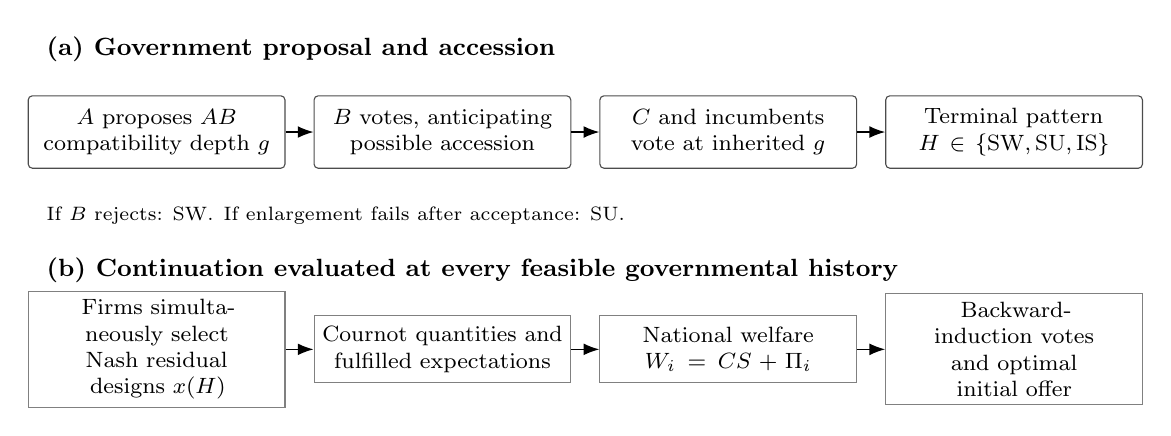
\begin{tikzpicture}[x=1cm,y=1cm,>=Latex,
    gov/.style={draw=black!70,rounded corners=1.5pt,align=center,
      text width=3.05cm,minimum height=0.92cm,font=\footnotesize,inner sep=3pt},
    econ/.style={draw=black!50,align=center,text width=3.05cm,
      minimum height=0.85cm,font=\footnotesize,inner sep=3pt},
    arrow/.style={-{Latex[length=2mm]},line width=.45pt}]
\node[anchor=west,font=\small\bfseries] at (0,1.05) {(a) Government proposal and accession};
\node[gov] (a) at (1.52,0) {$A$ proposes $AB$\\compatibility depth $g$};
\node[gov] (b) at (5.15,0) {$B$ votes, anticipating\\possible accession};
\node[gov] (c) at (8.78,0) {$C$ and incumbents\\vote at inherited $g$};
\node[gov] (h) at (12.41,0) {Terminal pattern\\$H\in\{\SW,\SU,\IS\}$};
\draw[arrow] (a.east) -- (b.west);
\draw[arrow] (b.east) -- (c.west);
\draw[arrow] (c.east) -- (h.west);
\node[font=\scriptsize,anchor=west] at (0,-1.06) {If $B$ rejects: $\SW$. If enlargement fails after acceptance: $\SU$.};
\node[anchor=west,font=\small\bfseries] at (0,-1.75) {(b) Continuation evaluated at every feasible governmental history};
\node[econ] (x) at (1.52,-2.76) {Firms simultaneously select\\Nash residual designs $x(H)$};
\node[econ] (q) at (5.15,-2.76) {Cournot quantities and\\fulfilled expectations};
\node[econ] (w) at (8.78,-2.76) {National welfare\\$W_i=CS+\Pi_i$};
\node[econ] (v) at (12.41,-2.76) {Backward-induction votes\\and optimal initial offer};
\draw[arrow] (x.east) -- (q.west);
\draw[arrow] (q.east) -- (w.west);
\draw[arrow] (w.east) -- (v.west);
\end{tikzpicture}
\caption{Game timing and the role of continuation payoffs. Governments specify a possible compatibility pattern and depth; for each contemplated terminal pattern firms select residual designs before Cournot competition. Governments anticipate these continuation payoffs when voting. The baseline does not permit renegotiation of $g$ at accession.}
\label{fig:timing}
\end{figure}

\section{Cournot equilibrium and private design response}\label{sec:equilibrium}
\subsection{Market-stage equilibrium and the no-agreement reference}
Since $B_{ii}=1$, firm $i$'s Cournot first-order condition at fixed expectations is $p_i-c=q_i$. Imposing fulfilled expectations $\bar q=q$ gives
\begin{equation}\label{eq:cournot}
M q=d\vect{1},\qquad q=d M^{-1}\vect{1},
\end{equation}
provided $M$ is invertible and $q\gg0$. The expression defines outputs conditional on policy $H$ and design $x$. It is the interior continuation formula, not by itself a global design-equilibrium certificate.

Write the useful abbreviations
\begin{equation}\label{eq:abbrev}
\alpha=2-\eta,\quad\beta=1-\rho,\quad\delta=\rho-\eta,\quad
t=\beta z,\quad P=\alpha-t,\quad L=\alpha+2t.
\end{equation}
At fragmentation the symmetric interior design Nash $z$ obeys
\begin{equation}\label{eq:root}
\kappa(1-z)=\frac{6\beta\alpha d^2}{(\alpha-t)L^3},\qquad t=\beta z,\qquad q_0=\frac dL.
\end{equation}
The solution on the certified branch has $0<z<1$ and $P,L>0$. The derivation uses the \emph{unilateral} firm-design first-order condition; treating the firms as a common social planner would yield a different equation.

\subsection{The implicit Nash response rather than a planner response}
Let $F_i(x;H)=\partial\Pi_i(x;H)/\partial x_i$ be firm $i$'s own design derivative, already anticipating the quantity equilibrium in \eqref{eq:cournot}. The private Nash system is
\begin{equation}\label{eq:designFOC}
F_i(x;H)=0\quad (i=A,B,C).
\end{equation}
Where the full $3\times3$ Jacobian $J=\partial F/\partial x$ is nonsingular, the equilibrium design response to policy depth is
\begin{equation}\label{eq:implicit}
\frac{dx}{dg}=-J^{-1}\frac{\partial F}{\partial g}.
\end{equation}
This response incorporates the strategic adjustment of rival firms. It cannot be replaced by three independent optimizations holding their competitors' designs fixed. Similarly, each firm's private FOC annihilates the derivative of \emph{its own} profit with respect to \emph{its own} chosen design, but neither the effect on domestic consumers nor the effect of competitors' designs on its worldwide profit. This distinction generates our main incidence term.

\section{The national-incidence mechanism}\label{sec:mechanism}
\subsection{Symmetry turns one edge into an accession constraint}
For the derivative analysis, allow the three compatibility edges $e_{AB}$, $e_{AC}$, $e_{BC}$ to vary separately near zero. The firm continuation and national reduced payoffs inherit the permutation symmetry of the primitive game.
\begin{lemma}[Edge incidence]\label{lem:edges}
Assume differentiable, unique symmetric firm continuations at fragmentation. There exist numbers $\mu$ and $\nu$ such that a country's marginal welfare response to an incident compatibility edge is $\mu$, and its response to the remaining nonincident edge is $\nu$. Consequently,
\begin{equation}\label{eq:edges}
m'(0)=\mu,\quad o'(0)=\nu,\quad i'(0)=2\mu+\nu,\quad
[i-o]'(0)=2\mu,\quad [i-m]'(0)=\mu+\nu.
\end{equation}
The identities apply separately under endogenous and frozen residual design.
\end{lemma}
\begin{proof}
Differentiate each country's reduced welfare with respect to the three independently variable edges at zero. Permuting country labels leaves the game invariant. For any country, the two incident edges therefore have a common coefficient $\mu$, and the third edge has coefficient $\nu$. A bilateral $AB$ link activates one edge; a common-depth grand standard activates all three. Taking directional derivatives and subtracting gives \eqref{eq:edges}.
\end{proof}

The lemma is a symmetry accounting identity, not a new economic discovery. Its use here is to show exactly why a member's marginal incentive also determines the outsider's \emph{accession} comparison. The incumbent and outsider votes are distinct government comparisons, but their first-order effects are linked by the three-country structure.

\subsection{What private redesign subtracts from national welfare}
Define the \emph{frozen-design} counterfactual by keeping every $x_i=z$, its actual no-agreement Nash value, at all positive-depth policy histories. Firms still compete in the Cournot market, governments still optimize the initial depth, and the accession and rejection rules are unchanged. Let subscript $\F$ denote these payoffs and $\N$ the fully endogenous design payoffs. At $g=0$ both regimes coincide.

An $AB$ link at fixed $x=z$ yields the bilateral-member national welfare slope
\begin{equation}\label{eq:D}
D\equiv\mu_{\F}=
\frac{\rho d^2}{L^2}-\frac{\delta d^2}{L^3}
\left(2(1+2t)+\frac{6\alpha}{P}\right).
\end{equation}
This combines a direct compatibility-related consumer gain with the effects of output adjustment on consumer surplus and on the home firm's profits. The outsider's frozen-design response is
\begin{equation}\label{eq:nuF}
\nu_{\F}=\frac{\rho d^2}{L^2}-\frac{2\delta d^2(1+2t)}{L^3}
+\frac{12\delta d^2t}{PL^3}.
\end{equation}
With endogenous design, symmetry of $AB$ implies two relevant slopes, $u'=dx_A^{\SU}/dg|_0=dx_B^{\SU}/dg|_0$ and $v'=dx_C^{\SU}/dg|_0$, determined by \eqref{eq:implicit}.

The derivative of $A$'s \emph{national welfare}, evaluated at the no-agreement private Nash, satisfies
\begin{equation}\label{eq:Wgrad}
\partial_{x_A}W_A=-C,\qquad
\partial_{x_B}W_A=\partial_{x_C}W_A=-(C+V),
\end{equation}
where
\begin{equation}\label{eq:CV}
C=\frac{\beta d^2(\eta+2t)}{L^3},\qquad
V=\frac{3\beta d^2(\alpha-2t)}{PL^3}.
\end{equation}
Here $C$ summarizes the consumer-side incidence, while $V$ captures the incremental worldwide home-profit response to \emph{other firms'} choices. Neither should be removed by invoking firm $A$'s own-profit FOC.

\begin{lemma}[National-welfare incidence of noncooperative design]\label{lem:incidence}
Under regular interior firm design Nash and the maintained primitives, the endogenous bilateral-member derivative is
\begin{equation}\label{eq:loss}
\mu_{\N}=D-\loss,\qquad
\loss\equiv C(2u'+v')+V(u'+v').
\end{equation}
In particular, $C,V,u',v'>0$ implies $\loss>0$. If $0<D<\loss$, a member gains from a marginal compatibility link under frozen design but loses after noncooperative redesign.
\end{lemma}
\begin{proof}
Apply the chain rule to $W_A(g,x^\SU(g))$ at zero. Its fixed-design part is $D$ by \eqref{eq:D}. The Nash-adjustment part is $\partial_x W_A\cdot(u',u',v')$, which by \eqref{eq:Wgrad} equals $-C(2u'+v')-V(u'+v')$. This establishes \eqref{eq:loss}. Positivity yields the final inequality. The derivative of the own optimized \emph{private profit} with respect to $x_A$ vanishes, but its domestic consumer effect and the response to rivals' designs do not; omitting the $V$ term changes the conclusion and is incorrect.
\end{proof}

\paragraph{Economic interpretation.}
There is no general welfare envelope theorem for a government when firms privately optimize product positions. Standardization changes the privately desirable residual characteristics. A firm has no incentive to internalize every resident consumer's lost surplus, nor the effect of competitors' adjustments on its export profits. A sufficiently strong induced response therefore destroys a government gain that would have been present if product attributes were constrained. Our analytical innovation is the \emph{incidence and policy comparison within this particular two-level game}, not the abstract chain rule $D-\loss$ alone.

Figure~\ref{fig:mechanism} summarizes the identifying experiment: no policy primitive or government voting rule changes between the frozen and endogenous-design cases.


\begin{figure}[tbp]
\centering
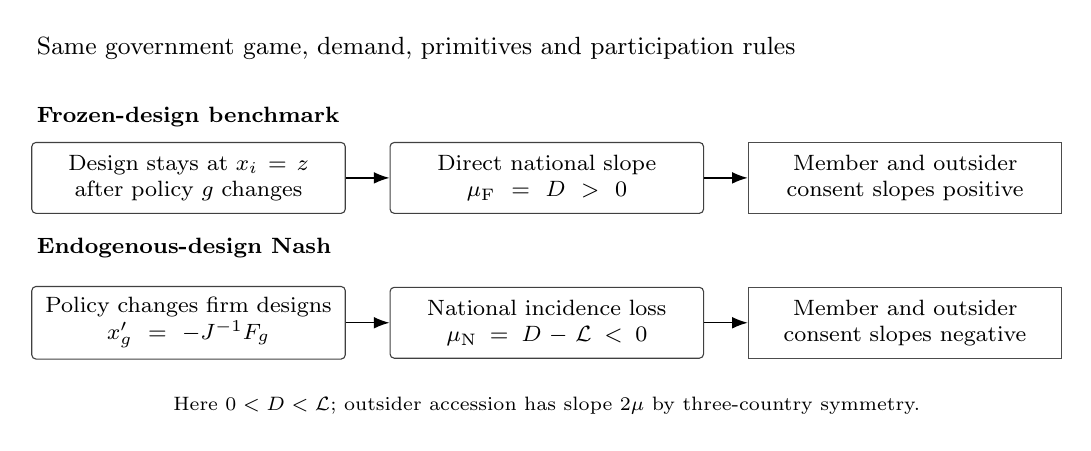
\begin{tikzpicture}[x=1cm,y=1cm,>=Latex,
    mech/.style={draw=black!75,rounded corners=1.5pt,align=center,font=\footnotesize,
       minimum height=0.9cm,text width=3.7cm,inner sep=4pt},
    answer/.style={draw=black!70,align=center,font=\footnotesize,
       minimum height=0.9cm,text width=3.7cm,inner sep=4pt},
    arrow/.style={-{Latex[length=2mm]},line width=.5pt}]
\node[font=\small,anchor=west] at (-0.05,1.45) {Same government game, demand, primitives and participation rules};
\node[font=\footnotesize\bfseries,anchor=west] at (-0.05,0.57) {Frozen-design benchmark};
\node[mech] (f1) at (2.0,-0.20) {Design stays at $x_i=z$\\after policy $g$ changes};
\node[mech] (f2) at (6.55,-0.20) {Direct national slope\\$\mu_{\F}=D>0$};
\node[answer] (f3) at (11.1,-0.20) {Member and outsider\\consent slopes positive};
\draw[arrow] (f1.east) -- (f2.west);
\draw[arrow] (f2.east) -- (f3.west);
\node[font=\footnotesize\bfseries,anchor=west] at (-0.05,-1.09) {Endogenous-design Nash};
\node[mech] (n1) at (2.0,-2.04) {Policy changes firm designs\\$x'_g=-J^{-1}F_g$};
\node[mech] (n2) at (6.55,-2.04) {National incidence loss\\$\mu_{\N}=D-\mathcal L<0$};
\node[answer] (n3) at (11.1,-2.04) {Member and outsider\\consent slopes negative};
\draw[arrow] (n1.east) -- (n2.west);
\draw[arrow] (n2.east) -- (n3.west);
\node[font=\scriptsize,align=center] at (6.55,-3.09)
 {Here $0<D<\mathcal L$; outsider accession has slope $2\mu$ by three-country symmetry.};
\end{tikzpicture}
\caption{Controlled causal comparison at the no-agreement boundary. Private redesign affects both domestic consumer surplus and the home firm's worldwide profits; the private firm's own first-order condition does not eliminate this national incidence. The diagram summarizes the \emph{local} sign result, not a general theorem of agreement failure under every bargaining protocol.}
\label{fig:mechanism}
\end{figure}

\section{Main result: private redesign reverses governmental consent}\label{sec:global}
\begin{theorem}[Local controlled participation reversal]\label{thm:local}
Suppose the firm continuation is regular, unique, interior, and continuously differentiable near fragmentation, and suppose the primitive parameters imply $\beta>0$, $\rho>\eta$, $C,V,u',v'>0$ and
\begin{equation}\label{eq:conditions}
0<D<\loss,\qquad \nu_{\N}>-2\mu_{\N},\qquad \nu_{\F}>-D.
\end{equation}
For every sufficiently small $g>0$, (a) with frozen design the inherited-depth procedure has affirmative bilateral-member and outsider-accession votes, and an acceptable integrated agreement strictly improves on fragmentation; (b) with endogenous design, the bilateral-member and outsider-accession conditions fail while the hypothetical integrated allocation at the same depth strictly Pareto-improves on fragmentation. The statement is local in $g$; it does not alone establish the government-optimal regime over all depths.
\end{theorem}
\begin{proof}
By Lemma~\ref{lem:incidence}, $\mu_{\F}=D>0$ but $\mu_{\N}=D-\loss<0$. Lemma~\ref{lem:edges} gives the frozen outsider accession slope $[i_{\F}-o_{\F}]'(0)=2D>0$ and incumbent widening slope $[i_{\F}-m_{\F}]'(0)=D+\nu_{\F}>0$. The frozen grand benefit slope is $2D+\nu_{\F}>0$. In the endogenous game, $m_{\N}'(0)=\mu_{\N}<0$ and $[i_{\N}-o_{\N}]'(0)=2\mu_{\N}<0$, whereas $i_{\N}'(0)=2\mu_{\N}+\nu_{\N}>0$. Each compared level gap is zero at $g=0$. Strict derivative inequalities and differentiability therefore imply the specified level inequalities for all sufficiently small positive $g$. The government's comparison in \eqref{eq:consent} then produces the stated local voting outcomes.
\end{proof}

The theorem rules out an alternative explanation based only on changing government commitments across the two main experiments: the same governments have the same admissible proposal and voting game. The change is the privately optimized continuation $x_i$. Yet the theorem should not be described as a general impossibility of integration, for the separate agenda comparison below shows how the institutional restriction matters.

\begin{theorem}[An open primitive region with different government-optimal outcomes]\label{thm:open}
There exists a nonempty open neighborhood $\mathcal U$ of
\begin{equation}\label{eq:theta}
\theta_0=(d,\eta,\rho,\kappa)=\left(1,\frac{379}{500},\frac9{10},\frac{1701}{2000}\right)
\end{equation}
in the four-dimensional baseline primitive parameter space such that the following hold in the maintained inherited-depth game:
\begin{enumerate}
\item With endogenous firm design, every strictly positive-depth proposal fails the original accession procedure; the government-optimal equilibrium regime is fragmentation $\SW$.
\item With all residual designs fixed at their \emph{same} no-agreement Nash $z$, a strictly positive-depth integrated agreement is approved and yields a higher initiating-country payoff than any terminal bilateral arrangement or fragmentation; hence a government-optimal positive $\IS$ proposal exists.
\item For these primitives, some hypothetical direct integrated agreement under endogenous design strictly improves the national welfare of all three countries relative to $\SW$.
\end{enumerate}
This does not assert an explicit radius for $\mathcal U$, an all-parameter global classification, or coalition-proof fragmentation.
\end{theorem}
\begin{proof}[Proof architecture and certified bounds]
At $\theta_0$, the historical Stage-14 all-depth interval certificates establish, for $g\in[0,1]$, strict derivative \emph{upper} bounds
\begin{equation}\label{eq:cert}
\frac{dm_{\N}}{dg}<-0.0079701929973,\qquad
\frac{d(i_{\N}-o_{\N})}{dg}<-0.0150388833377.
\end{equation}
The underlying checks include the unique full-firm Nash continuation, positive quantities, regularity and enclosure of the derivative along the full policy-depth interval; they are not merely a local FOC calculation. Integrating from $g=0$, where all regime welfare levels coincide, yields $m_{\N}(g)<s$ and $i_{\N}(g)<o_{\N}(g)$ at every $g>0$. Thus neither an accepted $\SU$ nor an enlargement to $\IS$ survives the original voting conditions; optimizing over the full depth menu returns $\SW$.

For the frozen-design game, the previously certified all-depth bilateral payoff bound and the strictly feasible integrated candidate at $g=1/20$ give
\begin{equation}\label{eq:frozenCert}
 i_{\F}(1/20)>2.4413970373,
\quad s<2.4220784218,
\quad\sup_{0\le g\le1}m_{\F}(g)<2.4235735642,
\end{equation}
while $i_{\F}(1/20)>o_{\F}(1/20)$ and $i_{\F}(1/20)>m_{\F}(1/20)$ strictly. The candidate is accepted, beats $\SW$, and beats the entire terminal bilateral payoff envelope, so an optimal accepted positive-depth integrated offer exists. Separately the actual endogenous integrated outcome at $g=1/20$ satisfies $i_{\N}(1/20)-s>0.0169346278736$.

The all-depth strict inequalities, positive-output margins and uniform full-cube equilibrium-uniqueness/regularity margins survive under sufficiently small primitive perturbations. A finite-cover implicit-function argument, continuity of derivatives on a compact depth interval, and the maximum theorem preserve strict negative endogenous slopes and the strict frozen integrated-versus-bilateral envelope gap. The local no-agreement and positive-depth inequalities thereby hold on some common \emph{open} neighborhood $\mathcal U$. The existence assertion is qualitative; no explicit primitive box is supplied. The complete numerical certification targets, algorithms, and audit provenance must be supplied as machine-readable supplementary material at submission (Appendix~\ref{app:cert}).
\end{proof}

\paragraph{Why this is stronger than a calibrated sign example.}
The local inequality $0<D<\loss$ identifies the source of the change; the all-depth bound rules out a compensating proposal at some other $g$. The open-neighborhood argument, rather than one isolated numerical parameter choice, rules out a pure knife-edge arithmetic artifact. On the other hand, the open neighborhood does \emph{not} establish robustness to a different bargaining procedure, demand function, or number of countries.

Table~\ref{tab:map} distinguishes the main reversal from the institutional and parameter-boundary results; it also records where the proofs are local, all-depth or restricted to a limiting family.


\begin{table}[tbp]
\centering\footnotesize
\caption{Hierarchy, proven domains, and limits of the results}\label{tab:map}
\renewcommand{\arraystretch}{1.22}
\begin{tabularx}{\linewidth}{@{}>{\raggedright\arraybackslash}p{.18\linewidth}>{\raggedright\arraybackslash}p{.34\linewidth}>{\raggedright\arraybackslash}X@{}}
\toprule
Result & Proven environment or condition & Inference and scope limit \\
\midrule
Local reversal & $0<D<\mathcal L$, regular design Nash; additional outsider slope conditions & Frozen design gives positive consent slopes; endogenous design reverses both. \emph{Local} in $g$. \\
Global regime & Certified all-depth inequalities at $\theta_0$ and a nonempty open primitive neighborhood & $\SW$ with design Nash versus government-optimal $\IS$ with frozen design. Specific inherited-depth protocol; not coalition-proof. \\
Direct-grand & $\mu_{\N}<0<2\mu_{\N}+\nu_{\N}$ & Direct $\IS$ can benefit all at the same small $g$; procedural boundary, not a general new coalition theorem. \\
Design costs & $\lambda_c\in(0.93538,0.93539)$ at $\theta_0$ & Unique \emph{local} consent cutoff; no global $\lambda$ regime classification. \\
Network intensity & $\rho=1$, $\eta=6/7$ cutoff and restricted $\rho<1$ strip & Exact global regimes on the design-inactive face; only restricted nearby endogenous extension. \\
\bottomrule
\end{tabularx}
\end{table}

\subsection{An interpretable numerical illustration}
At $\theta_0$ the no-agreement symmetric private design is $z\simeq0.7185927073$. We obtain $D\simeq0.0067679241$, $\loss\simeq0.0150697441$ and $\mu_{\N}\simeq-0.0083018200$. For the same policy depth $g=0.05$, all values below are \emph{national welfare differences} from the corresponding bilateral, outsider, or fragmentation alternatives. Table~\ref{tab:effects} is based on the independently reconstructed Stage-23 equilibrium evaluator and is shown to explain magnitudes and signs; it does not replace the rigorous all-depth argument.
\begin{table}[ht]
\centering\small
\caption{Government welfare comparisons at $g=0.05$ (uncalibrated model units)}\label{tab:effects}
\begin{tabular}{lrrr}
\toprule
Firm-design treatment&$m-s$&$i-o$&$i-s$\\
\midrule
Frozen at original $z$&$+0.000272382$&$+0.000234617$&$+0.019318616$\\
Endogenous design Nash&$-0.000473474$&$-0.001246547$&$+0.016934628$\\
\bottomrule
\end{tabular}
\end{table}
The endogenous direct grand gain corresponds to approximately $0.70\%$ of the baseline welfare level in these \emph{non-calibrated} model units. We make no empirical claim that real-world gains have this size. The analytically relevant observation is the opposition between a positive grand gain and negative consent margins in the inherited-depth sequence.

Figure~\ref{fig:phase} maps the government-optimal terminal regime in the $(\kappa,\eta)$ plane, holding $d=1$, $\rho=0.9$ and the governmental voting procedure fixed. In Panel~(a), firms' designs are frozen at each parameter pair's own fragmentation Nash level $z(\kappa,\eta)$; in Panel~(b), firms reoptimize those designs following the anticipated policy choice. Both panels optimize the initiating government's depth $g$ over the same admissible policy menu. At the certified benchmark star, frozen design supports $\IS$ while endogenous design leads to $\SW$. This controlled comparison, rather than the exact appearance of a boundary line, is the figure's economic point. The plot is a numerical illustration on a $(41\times41)$ parameter lattice, with denser government-depth exploration near regime changes; it is not a two-dimensional interval-certificate theorem.

\paragraph{Why a bilateral-only region is not identified in this numerical slice.}
At any \emph{specified} depth, a bilateral $\SU$ requires $m(g)\ge s$ and at least one failed enlargement vote (either $i(g)<m(g)$ or $i(g)<o(g)$). Yet these inequalities establish only a \emph{terminal outcome conditional on the proposed depth}; they do not imply that the initiating government optimally selects such a depth instead of another depth yielding $\IS$. This distinction is numerically material. A coarse depth grid initially suggested very narrow $\SU$ bands, but in the updated search every such cell was reclassified as $\SW$ or $\IS$ once the $g$ grid was refined to 321 points. All 28 cells whose classifications changed between the 81-point and 321-point depth searches retained the refined classification on a 641-point recheck. We therefore do not display a verified $\SU$ region in Figure~\ref{fig:phase}. Its absence from this finite numerical slice is \emph{not} a proof that $\SU$ cannot arise under other primitive parameters or even between sampled points. No closed-form phase boundary, global two-dimensional parameter theorem, or absence-of-$\SU$ theorem is claimed.

\begin{figure}[H]
\centering
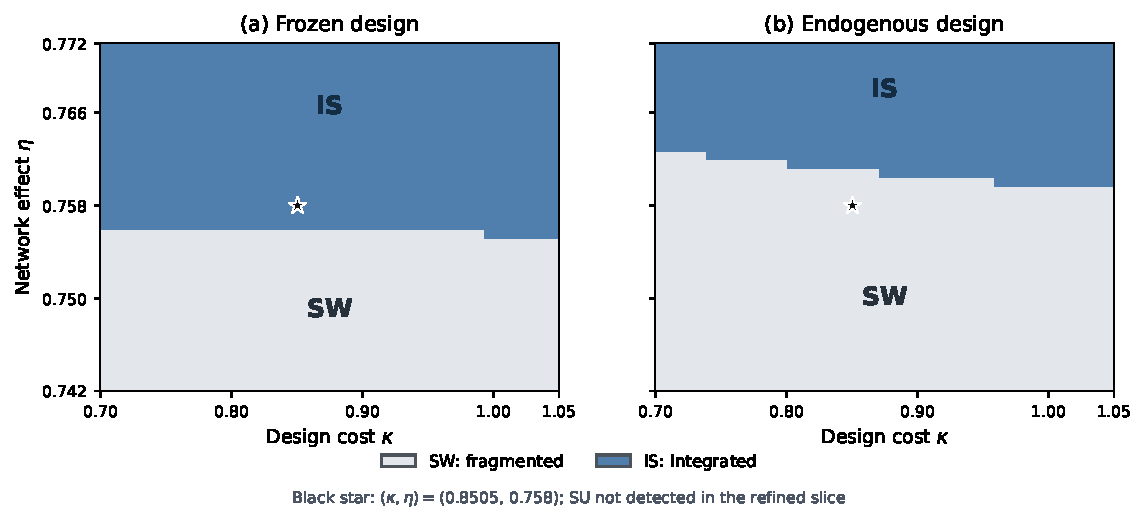
\includegraphics[width=0.96\linewidth]{figure3_v04_kappa_eta_phase.pdf}
\caption{Numerical government-regime map in the $(\kappa,\eta)$ plane. Both panels solve the same inherited-depth governmental game with $d=1$, $\rho=0.9$, and $\lambda=0$. Panel (a) fixes each parameter pair's private design at its own no-agreement Nash level; panel (b) allows Nash redesign after policy. Gray indicates fragmentation ($\SW$), blue a three-country agreement ($\IS$). A bilateral-only regime ($\SU$) was not detected in this refined slice. The star is the certified reference pair $(0.8505,0.758)$. Boundaries are numerical approximations, not theorem-certified phase curves.}
\label{fig:phase}
\end{figure}

\section{Negotiation routes and the meaning of institutional specificity}\label{sec:institution}
A natural objection is that a government could avoid the inherited bilateral accession path and instead offer a direct three-country agreement. That objection is correct: no bargaining-invariance or coalition-proof claim follows from our baseline model. We can nevertheless use it to separate the economic effect of private redesign from the effect of the accession protocol.

Consider an \emph{alternative} governmental agenda permitting a direct $\IS$ offer at depth $g$, with rejection returning all three countries to $\SW$. Firms play exactly the \emph{same} Nash continuation $x^{\IS}(g)$ and the same Cournot game as in the baseline; only the available governmental offer and rejection histories differ. A direct offer is unanimously acceptable when $i_{\N}(g)\ge s$.

\begin{proposition}[Institutional boundary: direct versus inherited-depth agreement]\label{prop:direct}
Suppose the endogenous continuation is regular and $\mu_{\N}<0<2\mu_{\N}+\nu_{\N}$. Then at every sufficiently small positive depth the baseline inherited-depth votes prevent a bilateral-first path from producing integration, while a \emph{direct} integrated proposal at the same depth is strictly Pareto-improving and accepted against fragmentation. At $\theta_0$, the baseline game returns fragmentation at every depth and at least one positive-depth direct proposal is strictly acceptable.
\end{proposition}
\begin{proof}
From Lemma~\ref{lem:edges}, $m_{\N}'(0)=\mu_{\N}<0$ and $[i_{\N}-o_{\N}]'(0)=2\mu_{\N}<0$, whereas $i_{\N}'(0)=2\mu_{\N}+\nu_{\N}>0$. All level gaps start at zero, yielding the local result. At $\theta_0$, Theorem~\ref{thm:open} establishes global failure under inherited depth, while the certified inequality $i_{\N}(1/20)>s$ establishes an accepted direct alternative. Existence of an optimal accepted direct offer follows from the compact policy menu and the maintained weak-acceptance rule.
\end{proof}

\paragraph{Interpreting the restriction.}
This proposition is not independently novel as a generic regional-versus-global coordination result: related barriers to multilateral standardization are established by \citet{Takarada2020} and \citet{Kawabata2021}. Its role is to specify the \emph{scope} of the main design-incidence result. In particular, it prevents the false inference that firms' redesign makes multilateral compatibility intrinsically unattractive.

A sequential accession institution is appropriate as a conditional model of a previously specified technical arrangement. Its depth $g$ is chosen in the initial proposal rather than fixed from the beginning of time; however, the terms are inherited during a subsequent accession decision. Technical revision might in practice require separate bargaining and compatibility testing. We do not assign such activities a quantitative cost in the baseline and therefore do not claim to derive its institutional commitment endogenously. \citet{Simcoe2012} documents bargaining-related delays in an actual standards committee, lending motivation to treating collective technical coordination as costly but not identifying our exact voting sequence.

If entrants and incumbents could jointly select a different depth $g'$ upon enlargement, a relevant feasibility condition would be $i_{\N}(g')\ge\max\{m_{\N}(g),o_{\N}(g)\}$ with an appropriate rejection continuation. Because $m_{\N}(g)$ and $o_{\N}(g)$ approach $s$ as $g\downarrow0$ whereas $i_{\N}(0.05)>s$ at the certified center, some sufficiently small inherited depth and a renegotiated $g'=0.05$ can satisfy these static consent inequalities. This is a \emph{feasibility comparison}, not a subgame-perfect solution of an unspecified renegotiation game. Transfers, renegotiation costs, binding commitment to future voting, and alternative coalition-formation rules are outside the modeled strategy space.

\section{Two boundaries: design adjustment and network effects}\label{sec:boundaries}
The main result uses no separate adjustment-cost parameter and holds with $\lambda=0$. Two previously established results delimit its scope. They are presented as conditional supporting analysis, not as independent broad discoveries.

\subsection{Costly redesign and a local consent threshold}
Let $z$ continue to denote the original no-agreement Nash characteristic and consider the explicit, separate extension
\begin{equation}\label{eq:lambda}
K_i(x_i;\lambda)=\frac{\kappa}{2}(1-x_i)^2+\frac{\lambda}{2}(x_i-z)^2,\qquad \lambda\ge0.
\end{equation}
Because the adjustment term vanishes to first order at $x_i=z$, the fragmentation Nash is unchanged. At $\theta_0$, let $\ell$ denote the diagonal entry of the design pseudo-gradient Jacobian, $\chi$ its common off-diagonal, and let $(p,p,r)$ be the derivative forcing from the $AB$ edge. The exact formulas are supplied in Appendix~\ref{app:lambda}. For $A_\lambda=\lambda-\ell$ and $\Delta_\lambda=(A_\lambda+\chi)(A_\lambda-2\chi)>0$,
\begin{equation}\label{eq:lambdaResp}
u'_\lambda=\frac{A_\lambda p+\chi r}{\Delta_\lambda},\qquad
v'_\lambda=\frac{2\chi p+(A_\lambda-\chi)r}{\Delta_\lambda}.
\end{equation}
Here $u'_\lambda$ denotes the member's design response, whereas $\nu_\lambda$ elsewhere denotes the \emph{outsider welfare} derivative; they are distinct objects.

\begin{proposition}[Unique \emph{local} design-friction cutoff]\label{prop:lambda}
At $\theta_0$, the marginal induced welfare loss $\loss(\lambda)=C(2u'_\lambda+v'_\lambda)+V(u'_\lambda+v'_\lambda)$ is strictly decreasing in $\lambda\ge0$ and converges to zero. Consequently there is a unique $\lambda_c>0$ satisfying $\loss(\lambda_c)=D$, certified by $0.93538<\lambda_c<0.93539$. The initial member and outsider accession slopes are negative for $0\le\lambda<\lambda_c$ and positive for $\lambda>\lambda_c$, locally near $g=0$, under the existing regularity conditions. No global equilibrium classification is claimed at $\lambda=\lambda_c$ or for all $\lambda>\lambda_c$.
\end{proposition}
\begin{proof}
At the certified primitive root, $Q_\lambda=-J(0)+\lambda I$ is a strictly diagonally dominant nonsingular $M$-matrix with $Q_\lambda^{-1}$ componentwise positive and positive forcing $f=(p,p,r)$. The equilibrium response is $Q_\lambda^{-1}f$ and satisfies $d(Q_\lambda^{-1}f)/d\lambda=-Q_\lambda^{-2}f\ll0$. Since $C,V>0$, the induced loss is positive, strictly decreasing, and tends to zero. Its value at zero exceeds $D>0$. The intermediate value theorem and strict monotonicity yield a unique threshold; the cited interval is from exact arithmetic. Lemma~\ref{lem:edges} turns the sign of $D-\loss(\lambda)$ into the first-order member and outsider vote signs. The result does not equate local vote feasibility with globally government-optimal $\IS$.
\end{proof}

\subsection{A network boundary, and what it cannot establish}
At $\rho=1$ the residual design $x_i$ drops out of cross-product compatibility and the baseline optimum is $x_i=1$ everywhere. Therefore this boundary is \emph{not} itself an example of private redesign. Nevertheless, the government game is analytically tractable and illustrates an exact boundary to the agreement regime.

Set $\vartheta=(1-\eta)/(2-\eta)$ and $E=d^2/(2-\eta)^2$. Direct solution yields
\begin{equation}\label{eq:face}
\begin{split}
s&=\tfrac92E,\\
m(g)&=E\left[\frac{4+g}{(1+\vartheta g)^2}+\tfrac12\right],\\
o(g)&=E\left[\frac{1+g}{(1+\vartheta g)^2}+\tfrac72\right],\\
i(g)&=E\frac{\tfrac92+3g}{(1+2\vartheta g)^2}.
\end{split}
\end{equation}
In particular,
\begin{equation}\label{eq:faceSign}
m(g)-s=E\frac{g(1-8\vartheta-4\vartheta^2g)}{(1+\vartheta g)^2}.
\end{equation}
The certified complete government-regime comparison on this \emph{limiting family} selects $\SW$ for $\eta\le6/7$ and a government-optimal $\IS$ for $\eta>6/7$; a positive-depth $\SU$ is never the optimal terminal regime. A restricted strip with genuinely active design exists for $\rho<1$ sufficiently close to 1 and has an implicit cutoff $\eta_c(\rho)$ with $\eta_c(1)=6/7$. The local expansion from earlier analysis is
\begin{equation}\label{eq:cutoffExpansion}
\eta_c(\rho)=\frac67+\frac{211}{196}(\rho-1)+O\big((1-\rho)^2\big),\quad \rho\uparrow1.
\end{equation}
No universal cutoff $6/7$ is claimed when $\rho<1$; no result here classifies arbitrary market primitives. This network boundary is secondary to the national-incidence mechanism.

\section{Relationship to the literature and interpretation}\label{sec:literature}
\citet{GandalShy2001} and \citet{Klimenko2009} develop international approaches to compatibility, network effects and strategic standards. In national standards policy, \citet{Costinot2008} shows how institutional rules affect the welfare consequences of domestic standards. Most directly, \citet{Takarada2020} studies regional and multilateral standards coalitions in a three-country model and finds that globally desirable cooperation need not be coalition-stable. \citet{Kawabata2021} establishes that harmonization in a deep regional trade agreement can impede multilateral free trade with an international standard. These are economic predecessors of our institutional comparison: failure of multilateral standardization is \emph{not} new per se.

\citet{Grossman2021} demonstrates how governments' regulatory commitments interact with firms' privately chosen product attributes and adaptation costs. We consequently do not claim that introducing private design into international regulatory cooperation is new in general. The more precise comparison is in strategic timing and the national welfare incidence: here the \emph{same} three-country governmental accession protocol is held fixed while privately optimal residual design is either permitted or frozen, which can change both member and outsider consent signs. This is a formal contribution within our stated network-Cournot environment; its broader economic priority and generality should not be exaggerated.

On the firm side, \citet{Buccella2023} characterizes compatibility strategies and endogenous choices in network industries, while \citet{Cheng2025} analyzes product quality, compatibility and veto. Their competitive incentive channels are relevant predecessors, but their verified main games place compatibility choice with firms, not with three welfare-maximizing governments followed by separate residual private design. In particular, a firm's compatibility cost or veto should not be identified with a government's consent constraint, or with the adjustment cost $\lambda$ in our extension. Details and unresolved full-text supplemental comparisons remain documented in the accompanying research ledger, rather than restated as unqualified priority claims.

An editor can still reasonably ask whether deriving a negative national incidence in this specific oligopoly adds enough economics beyond familiar investment and institutional commitment problems. Our answer cannot rest merely on a new derivative formula or the phrase ``compatibility may fail.'' The substantive increment is the controlled counterfactual and its globally certified regime switch: the same group of governments, with the same depth menu, reaches different agreement outcomes because private design changes the payoff from participation. The direct-grand case in Proposition~\ref{prop:direct} expressly states the limit of that finding.

\section{Conclusion}
International compatibility agreements can change firms' privately optimal residual product characteristics, not merely the attractiveness of their current products. The resulting design Nash can alter national welfare through domestic consumers and the home firm's worldwide earnings, and in a precisely characterized region it reverses governmental consent relative to a fixed-design benchmark. The sign reversal survives as a government-optimal regime difference on a certified nonempty open region of the model's baseline primitive parameters.

These findings do not imply universal noncooperation. Under the same economic environment, a direct integrated proposal can benefit all three countries, while the inherited-depth bilateral-first route fails. The paper therefore isolates a joint dependence on private adjustment and institutional commitment. It leaves unrestricted bargaining, endogenous protocol choice, renegotiation costs and empirical magnitudes to future research rather than treating those omitted features as already established.

\appendix
\section{Cournot inversion and the welfare-derivative bridge}\label{app:bridge}
At $\SW$ with $x_i=z$, the diagonal of $M$ is $\alpha$ and each off-diagonal entry is $t$. Thus
\begin{equation}\label{eq:inv}
M=P I+t\vect{1}\vect{1}^{\top},\qquad
M^{-1}=\frac1P\left(I-\frac{t}{L}\vect{1}\vect{1}^{\top}\right),\qquad q_0=\frac dL.
\end{equation}
Activating edge $AB$ while holding all $x=z$ changes $M$ in positions $(A,B)$ and $(B,A)$ by $\delta=\rho-\eta$. Differentiating $Mq=d\vect 1$ yields
\begin{equation}\label{eq:quantityDer}
\left.\frac{dq}{dg}\right|_{x=z,g=0}=-M^{-1}M_gq_0
=\left(-\frac{\delta\alpha q_0}{PL},-\frac{\delta\alpha q_0}{PL},\frac{2\delta t q_0}{PL}\right)^\top.
\end{equation}
Because $CS=\tfrac12q^\top Bq$, its total fixed-design derivative is
\begin{equation}\label{eq:CSder}
\left.\frac{dCS}{dg}\right|_{x=z,g=0}
=\frac{\rho d^2}{L^2}-\frac{2\delta(1+2t)d^2}{L^3}.
\end{equation}
The home firm of a member receives operating profit $3q_A^2$, so its fixed-design derivative is $6q_0(dq_A/dg)$. Combining it with \eqref{eq:CSder} gives \eqref{eq:D}. The outsider profit derivative $6q_0(dq_C/dg)$ similarly gives \eqref{eq:nuF}.

For clarity on the key correction, differentiating national welfare with respect to design $x_j$ differentiates both $B$ and quantities $q=dM^{-1}\vect{1}$. The $A$-firm FOC is $\partial_{x_A}\Pi_A=0$ at a private Nash but $\partial_{x_B}\Pi_A$ and $\partial_{x_C}\Pi_A$ need not vanish, nor does $\partial_{x_A}CS$. Direct differentiation and substitution of \eqref{eq:root} yield \eqref{eq:Wgrad}--\eqref{eq:CV}. Consequently the induced loss contains \emph{both} $C(2u'+v')$ and $V(u'+v')$, with the \emph{plus sign} shown in \eqref{eq:loss}. This displayed bridge is indispensable to the main theorem and must not be replaced by a black-box program output.

\section{Design-friction response and the critical coefficient}\label{app:lambda}
At $\theta_0$ and the unadjusted $\SW$ symmetric Nash let the diagonal and off-diagonal elements of $J(0)$ be $\ell$ and $\chi$. For the $AB$ edge, the forcing vector $f=(p,p,r)^{\top}$ is
\begin{align}
\ell&=-\kappa+\frac{6\beta^2d^2(\alpha-2t)(2\alpha+t)}{P^2L^4},
&\chi&=\frac{3\beta^2d^2(3\alpha-2t)}{PL^4},\\
p&=\frac{6\delta\beta d^2(\alpha-2t)(2\alpha+t)}{P^2L^4},
&r&=\frac{6\delta\beta d^2(\alpha^2-2\alpha t+4t^2)}{P^2L^4}.
\end{align}
At the exact interval bracket for the original $z$, $\ell<0$, $\chi,p,r>0$ and $-\ell>2\chi$. In the adjustment-cost extension $-J(\lambda)=-J(0)+\lambda I$, so
\[
\begin{pmatrix} A_\lambda-\chi &-\chi\\ -2\chi&A_\lambda\end{pmatrix}
\begin{pmatrix}u'_\lambda\\v'_\lambda\end{pmatrix}=
\begin{pmatrix}p\\r\end{pmatrix},\qquad A_\lambda=\lambda-\ell.
\]
Solving gives \eqref{eq:lambdaResp} and $\Delta_\lambda=(A_\lambda+\chi)(A_\lambda-2\chi)>0$. The strictly diagonally dominant nonsingular $M$-matrix argument in Proposition~\ref{prop:lambda} establishes monotonicity. At equality $\lambda=\lambda_c$ the first derivative vanishes; second-order terms must be analyzed before assigning a regime.

\section{Exact network-face identities and statement scope}\label{app:network}
On the limiting $\rho=1$ family, $\beta=0$ and residual private characteristics cannot affect $B$. Formulae \eqref{eq:face} solve the actual bilateral and integrated firm-production continuations. The numerator in \eqref{eq:faceSign} shows that a positive-depth bilateral offer is unprofitable when $\vartheta\ge1/8$, equivalently $\eta\le6/7$. The separate outsider-accession polynomial inequalities and, for $\eta>6/7$, the constructed accepted integrated offer beating the entire bilateral envelope are recorded in the certified Stage-21 theorem file. For $\rho<1$ close to 1, smooth Nash continuation plus uniform strict inequalities away from the boundary and a local second-order check yield the stated restricted endogenous strip. These are different mathematical claims: the exact face threshold is global on that face, while the continuation to active design is local in $\rho$ and does not have an arbitrary-$\rho$ formula.

\section{Computer-assisted global verification: auditable mapping}\label{app:cert}
Theorem~\ref{thm:open} incorporates \emph{previously obtained} all-depth certifications rather than claiming a new independent interval proof in this manuscript. The following records (relative to the relevant Stage-14, Stage-22, or Stage-23 repository directory), frozen at the corresponding earlier GitHub commit, must accompany the submission package and be checked against the precise text of the theorem:
\begin{itemize}
\item Stage 14, \texttt{canonical\_global\_rerun.log}: full-depth Krawczyk/derivative sign bounds and equilibrium regularity targets under $\theta_0$.
\item Stage 14, \texttt{pareto\_rerun.log}: exact enclosure of the direct integrated Pareto gain and frozen-design alternatives.
\item Stage 22, \texttt{STAGE22\_ABC\_PROPOSITIONS\_AND\_PROOFS.md}: theorem scope, center-primitive open-set proof and the analytic Jacobian/invariance bridges.
\item Stage 23, \texttt{stage23\_independent\_reconstruction.py}: clean-room local Nash/Cournot reconstruction, \texttt{stage23\_local\_reconstruction\_log.json}, and archived GitHub Actions run reproducing the historical all-depth code.
\end{itemize}
The interval proof must certify a \emph{full} private-design Nash rather than just a symmetric stationary root, positive Cournot quantities throughout $g\in[0,1]$, and uniform negative welfare-gap slopes. The open-neighborhood inference additionally uses uniform strict margins; an isolated positive/negative numerical calculation cannot replace it. All records should be incorporated into an immutable supplementary archive before submission. The source and article presently remain a \emph{research working draft}, not a submission-certified proof package.

\section*{Declarations (working-draft placeholders)}
\noindent\textbf{Funding and conflicts:} To be confirmed by the author before submission.\\
\textbf{Data and code availability:} Public research repository and reproducibility files will be linked to the exact frozen release upon submission.\\
\textbf{Use of AI assistance:} Material assistance in manuscript drafting and mathematical verification must be accurately disclosed under the eventual journal's current policy; all substantive results require author review and responsibility.\\
\textbf{Research status:} This draft has not been externally peer reviewed, and no final journal submission decision has been taken.

\begin{thebibliography}{99}\small
\bibitem[Buccella, Fanti and Gori(2023)]{Buccella2023} Buccella, D., Fanti, L., and Gori, L. (2023). Strategic product compatibility in network industries. \emph{Journal of Economics}, 140, 141--168. \url{https://doi.org/10.1007/s00712-023-00834-x}.
\bibitem[Cheng and Huang(2025)]{Cheng2025} Cheng, Y.-L., and Huang, H.-Y. (2025). Quality competition and product compatibility in network industries. \emph{Journal of Economics}, 145, 31--57. \url{https://doi.org/10.1007/s00712-024-00896-5}.
\bibitem[Costinot(2008)]{Costinot2008} Costinot, A. (2008). A comparative institutional analysis of agreements on product standards. \emph{Journal of International Economics}, 75, 197--213. \url{https://doi.org/10.1016/j.jinteco.2007.11.004}.
\bibitem[Gandal and Shy(2001)]{GandalShy2001} Gandal, N., and Shy, O. (2001). Standardization policy and international trade. \emph{Journal of International Economics}, 53, 363--383. \url{https://doi.org/10.1016/S0022-1996(00)00067-2}.
\bibitem[Grossman, McCalman and Staiger(2021)]{Grossman2021} Grossman, G. M., McCalman, P., and Staiger, R. W. (2021). The ``new'' economics of trade agreements: From trade liberalization to regulatory convergence? \emph{Econometrica}, 89, 215--249. \url{https://doi.org/10.3982/ECTA17536}.
\bibitem[Kawabata and Takarada(2021)]{Kawabata2021} Kawabata, Y., and Takarada, Y. (2021). Deep trade agreements and harmonization of standards. \emph{Southern Economic Journal}, 88, 118--143. \url{https://doi.org/10.1002/soej.12500}.
\bibitem[Klimenko(2009)]{Klimenko2009} Klimenko, M. (2009). Policies and international trade agreements on technical compatibility for industries with network externalities. \emph{Journal of International Economics}, 77, 151--166. \url{https://doi.org/10.1016/j.jinteco.2008.08.005}.
\bibitem[Simcoe(2012)]{Simcoe2012} Simcoe, T. (2012). Standard setting committees: Consensus governance for shared technology platforms. \emph{American Economic Review}, 102, 305--336. \url{https://doi.org/10.1257/aer.102.1.305}.
\bibitem[Takarada et~al.(2020)]{Takarada2020} Takarada, Y., Kawabata, Y., Yanase, A., and Kurata, H. (2020). Standards policy and international trade: Multilateralism versus regionalism. \emph{Journal of Public Economic Theory}, 22, 1420--1441. \url{https://doi.org/10.1111/jpet.12425}.
\end{thebibliography}
\end{document}
